%!TEX root = ../template.tex
%%%%%%%%%%%%%%%%%%%%%%%%%%%%%%%%%%%%%%%%%%%%%%%%%%%%%%%%%%%%%%%%%%%%
%% chapter5.tex
%% NOVA thesis document file
%%
%% Chapter with the robotic system description.
%%%%%%%%%%%%%%%%%%%%%%%%%%%%%%%%%%%%%%%%%%%%%%%%%%%%%%%%%%%%%%%%%%%%
\chapter{Robotic System}
\label{cha:robotic_system}

\begin{quotation}
\begin{flushright}
\itshape
«It's a lot like nuts and bolts - if the rider's nuts, the horse bolts!»\\
\textbf{- Nicholas Evans}
\end{flushright}
\end{quotation}

This chapter's goal is to describe in detail the robotic system used on this thesis. It will start with a general overview of the robot. It follows with a physical description of all the parts, safety considerations and installation procedure. The way to operate the robot and the operation limits will also be presented. The chapter will end with the description of the integrations with \gls{ros} and Gazebo.

% ==========================
% = Overview =
% ==========================

\section{Overview}
\label{sec:robotic_system_overview}

The robotic system is a robotic manipulator arm called Panda, from the german company Franka Emika GmbH (Fig. \ref{fig:franka_panda_overview}). It is an award winning robot in the category of collaborative robotics. It first won the Deutscher Zukunftspreis prize in 2017. On the following year, 2018, it also won the Time Best Inventions prize and German Innovation Award. In 2019, it won the iF Product Design Award \cite{FrankaEmikaGmbH_official_website}. 

\begin{figure}[htbp]
	\centering
	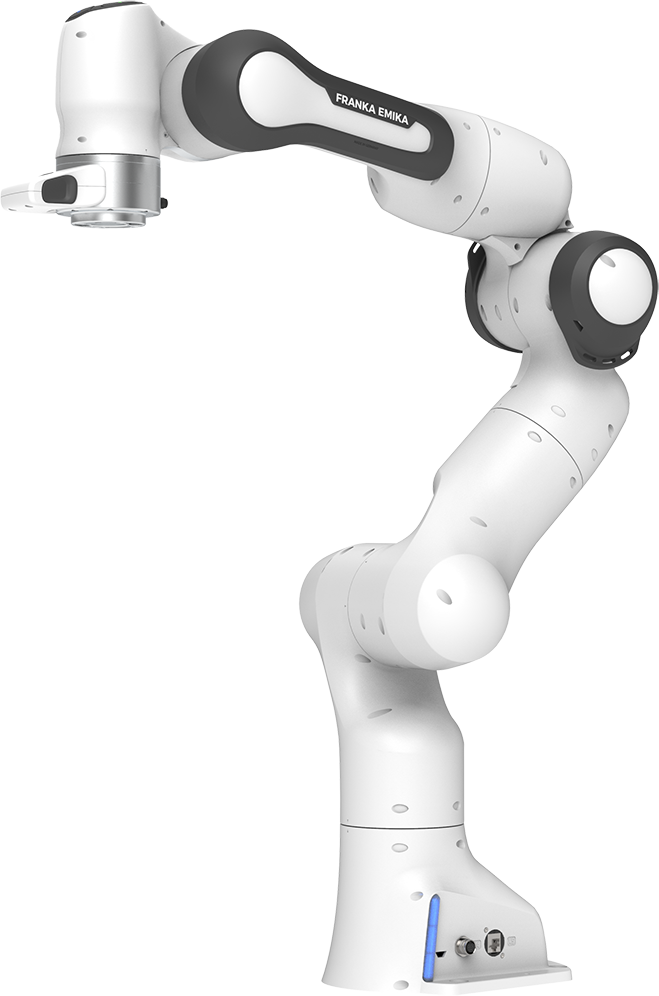
\includegraphics[width=.3\textwidth]{franka_panda_overview}
	\caption{Panda robotic manipulator arm from Franka Emika GmbH. Courtesy of Franka Emika GmbH, from the press kit available on \cite{FrankaEmikaGmbH_official_website}.}
	\label{fig:franka_panda_overview}
\end{figure}

The robot has seven degrees-of-freedom given from seven revolute joints. From a technology point-of-view, the joints are advanced mechatronic mechanisms. Each joint has a 14 bits resolution positional encoder. The motors used are a proprietary technology of brushless dc motors that are connected to strain wave gears for zero backlash. The joints also have torque sensors with 13 bits resolution. This complex joint system is controlled via real time electronics at 1 kHz rate \cite{FrankaEmikaGmbH_technology}.

The technology used on the joints contributes for the good operational results which robot has. Regarding free space motion the robot has a pose repeatabillity error of $\pm \SI{0.1}{\milli\meter}$ and a path deviation error of $\pm \SI{1.25}{\milli\meter}$. The torque sensors provide a resolution under 0.05 N on the forces measured at the end-effector. The force accuracy is 0.8 N and it has a repeatabillity under 0.05 N. The robot can apply forces to a minimum of 0.05 N at 1 kHz. Another characteristic of the robot is its collision detection capabilities. It can detect collisions in less than 2 ms, and react to it in less than 50 ms.

The robot versatility allows it to be used on a broad range of tasks. In a factory setting, it can be used for parts assembly, pick-and-place, and physical manipulation of tools. In conjunction with vision systems it can be used for visual inspection, sorting, and other vision-based tasks. Outside of the factory, these skills can be used to automate other processes that require the same skills. Another important point is that being a collaborative robot, it can work safely side-by-side with a human.

Besides all the physical capabilities, on the software side, the system comes with a web-based interface called \emph{Desk} to program the robot via apps. This system simplifies the configuration of specific tasks for the robot to execute. The tasks can be saved and even distributed across various robots. For research purposes, the robot comes with a control interface, \gls{fci}, that allows the user to create custom made controllers. This is the interface used on this thesis.

% section robotic_system_overview

% ==========================
% = Physical Description =
% ==========================

\section{Physical description}
\label{sec:robotic_system_physical_description}

The basic setup of the robot system is shown on Figure \ref{fig:robotic_system_basic_setup}. It shows the Panda \emph{Arm} with the \emph{Hand} end-effector. Along with it, there is the \emph{Control} hardware; the \emph{Host PC}, to connect to Desk and/or Control; and the security devices. Each one will be described in more detail.

\begin{figure}[htbp]
	\centering
	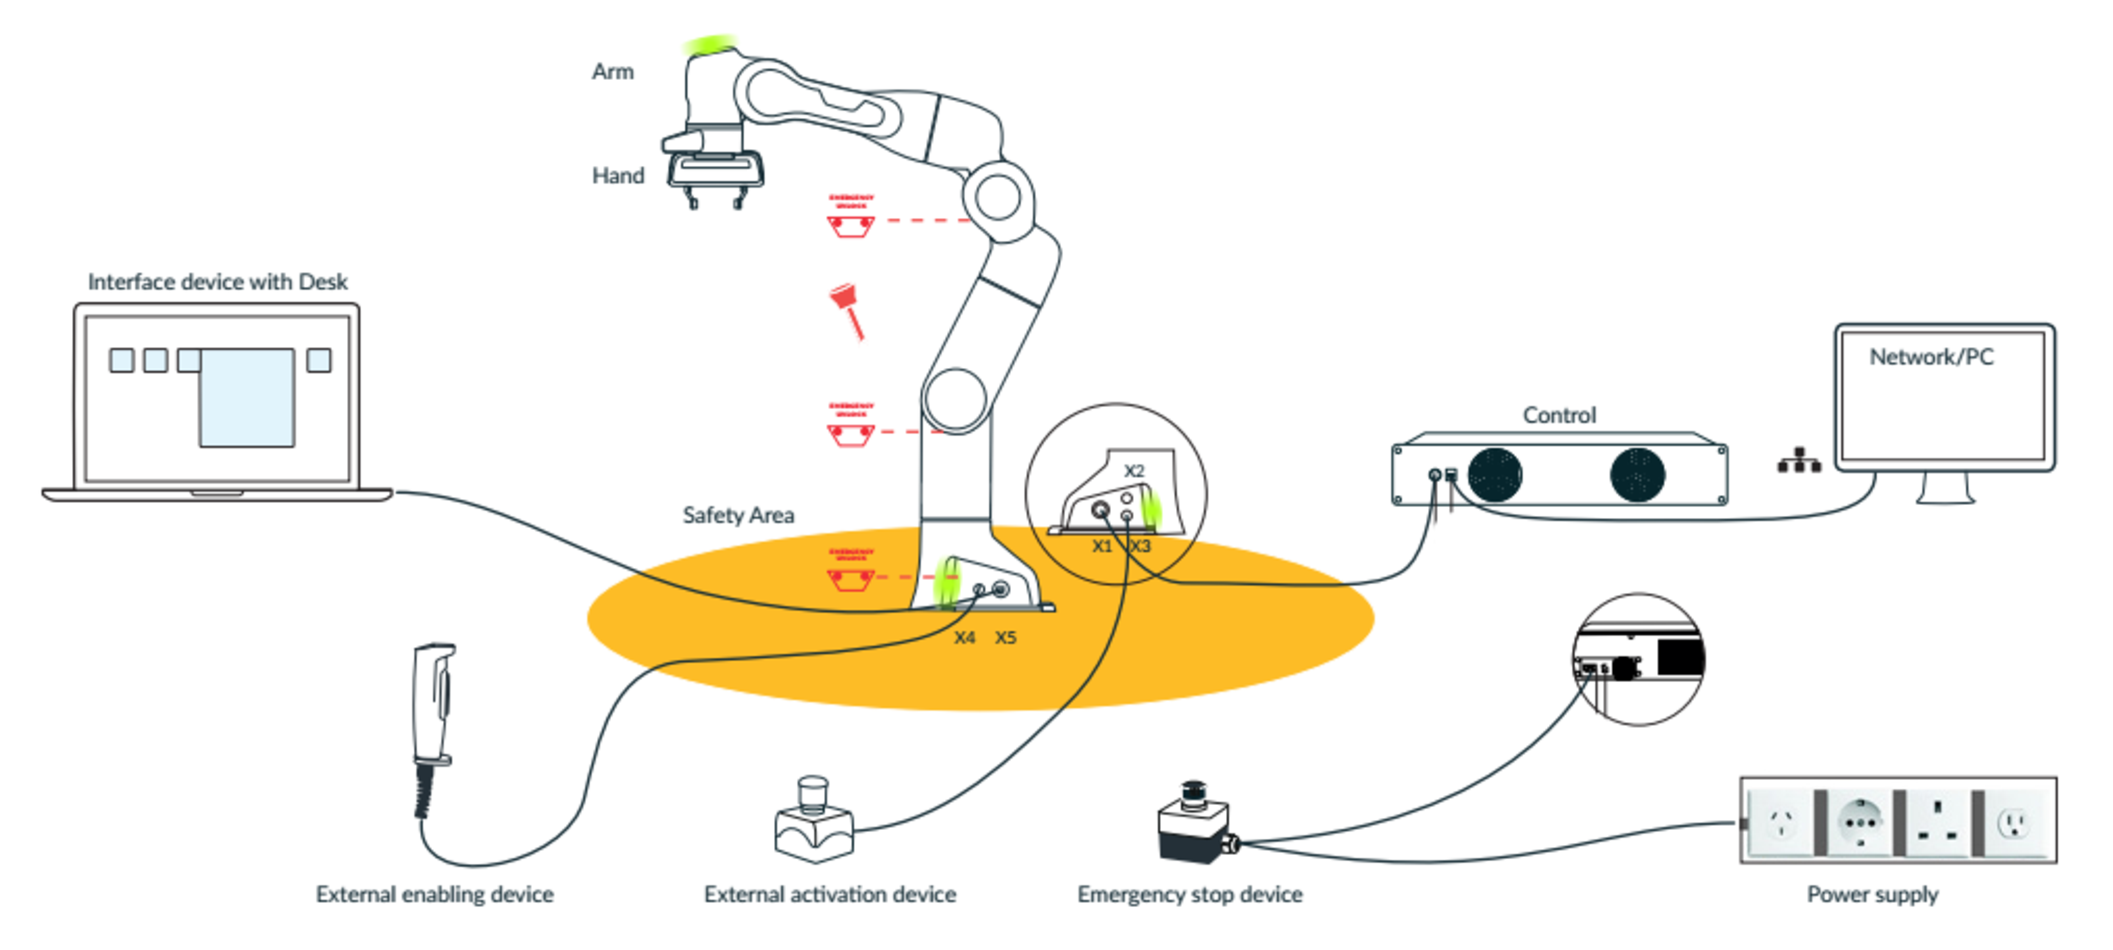
\includegraphics[width=\textwidth]{panda_basic_setup}
	\caption{Basic setup of the robotic system. Courtesy of Franka Emika GmbH and adapted from Panda user handbook of 2018.}
	\label{fig:robotic_system_basic_setup}
\end{figure}

\subsection*{Panda Arm}
\label{subsec:robotic_system_physical_description_panda_arm}

The Panda Arm is the main part of the robotic system. As previously mentioned, it has seven revolute joints, making it a redundant robot for any task in 3D space.

\begin{figure}[htbp]
	\centering
	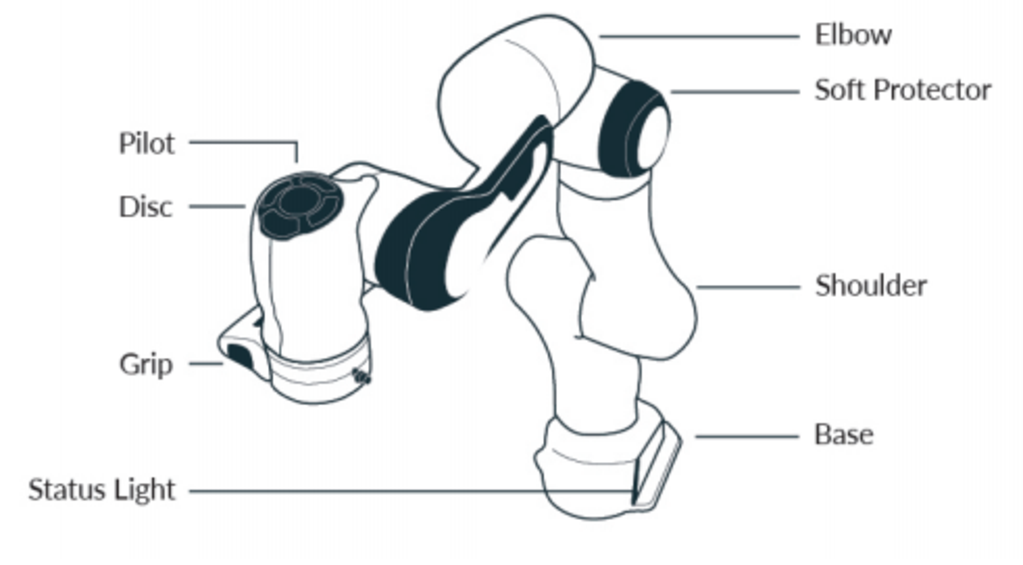
\includegraphics[width=0.8\textwidth]{panda_arm_components}
	\caption{Components of the Panda Arm. Courtesy of Franka Emika GmbH and adapted from Panda user handbook of 2018.}
	\label{fig:panda_arm_components}
\end{figure}

The Arm has several components worth mentioning (Fig. \ref{fig:panda_arm_components}). At the base of the robot there are two LED strip lights to indicate the status of the robot. These will be explained on section \ref{sec:robotic_system_operation}. Two of the joints have special names because of their resemblance to a human arm. The second joint is called \emph{Shoulder} and the fourth joint is called \emph{Elbow}. These are common joint names for anthropomorphic-like robot arms. The last link also has a special name, it is called \emph{Pilot}. It acts as a control platform for the robot. It works in conjunction with the Desk interface. The Pilot has the \emph{Disc} which is a set of control buttons, and the \emph{Grip}, which allows the user to manually guide the robot when in \emph{interactive} or "monitored stop" mode. The Pilot is show in more detail on Figure \ref{fig:panda_pilot_topview}.

\begin{figure}[htbp]
    \centering
	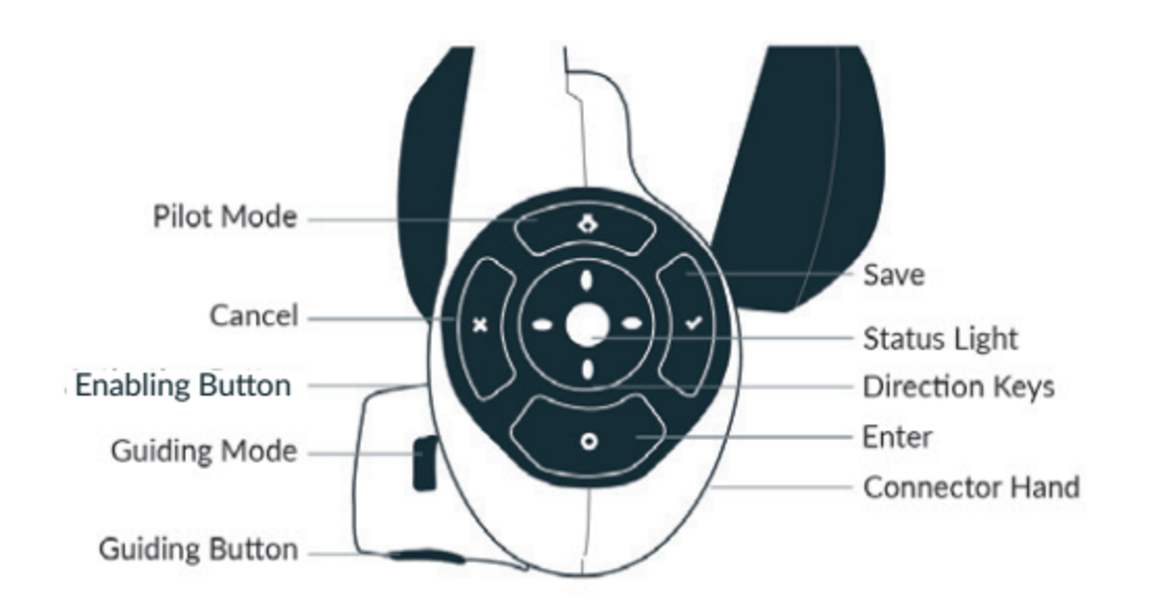
\includegraphics[width=0.8\textwidth]{panda_pilot_topview}
	\caption{Detailed view of Panda Arm Pilot. Courtesy of Franka Emika GmbH and adapted from Panda user handbook of 2018.}
	\label{fig:panda_pilot_topview}
\end{figure}

% subsection robotic_system_physical_description_panda_arm

\subsection*{Panda Hand}
\label{subsec:robotic_system_physical_description_panda_hand}

On a typical assembly of the Panda Arm, the end-effector used is the Panda Hand, which is the official end-effector. This tool is a two-finger, linear single axis robot hand (Fig. \ref{fig:panda_hand}). The Hand is powered directly from the Arm via a proprietary cable. The fingers can change positions in order to increase the span length. They can also be easily replaced by custom made fingers fitted for the task in hand. The fingertips can also be replaced in order to adapt the gripping format and strength to a specific task.

\begin{figure}[htbp]
    \centering
	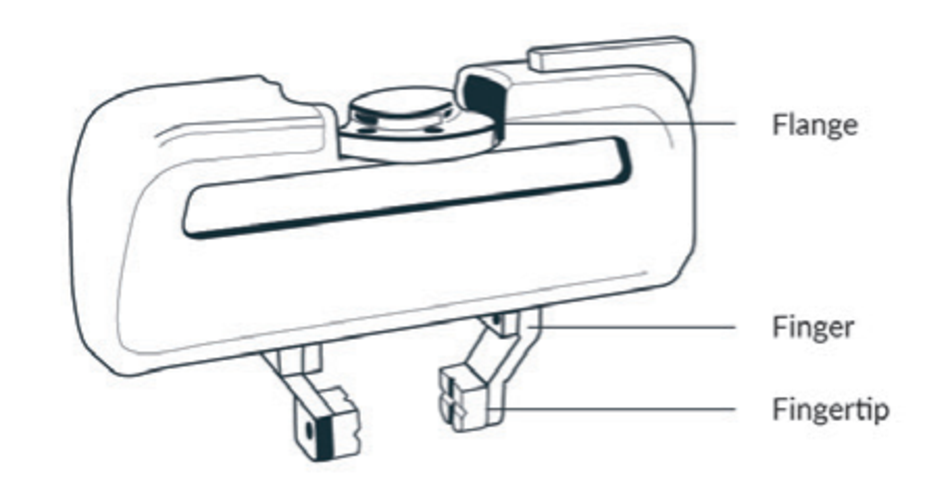
\includegraphics[width=0.8\textwidth]{panda_hand}
	\caption{Panda Hand. Courtesy of Franka Emika GmbH and adapted from Panda user handbook of 2018.}
	\label{fig:panda_hand}
\end{figure}

% subsection robotic_system_physical_description_panda_hand

\subsection*{Control}
\label{subsec:robotic_system_physical_description_control}

The Control is a special computer responsible for controlling the Panda Arm (Fig. \ref{fig:panda_control}). Without control the arm does not work. They are physically connected via a control cable. To control the robot via \gls{fci} the Host PC and the Control need to be connected via a RJ-45 ethernet cable. Otherwise, the Host PC can be directly connected to the Panda Arm base via the same cable.

\begin{figure}[htbp]
    \centering
	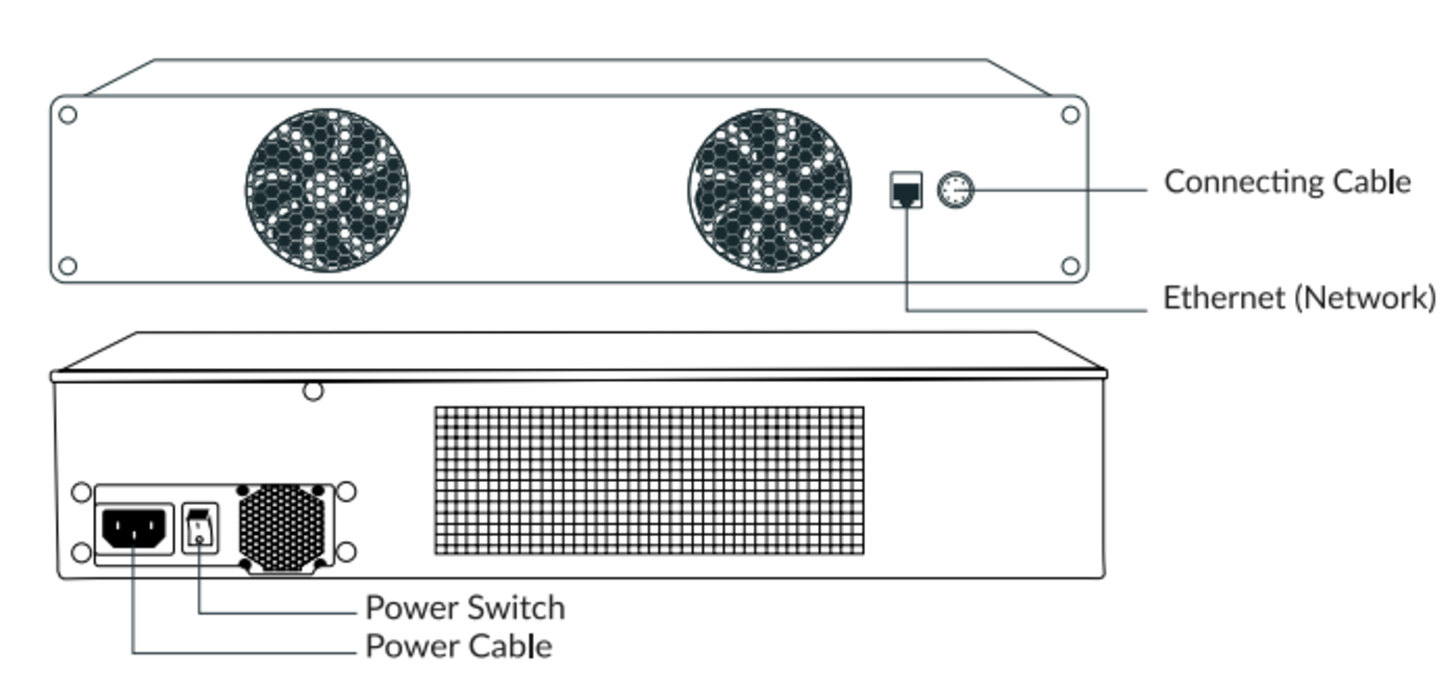
\includegraphics[width=0.8\textwidth]{panda_control}
	\caption{Panda Control hardware. Courtesy of Franka Emika GmbH and adapted from Panda user handbook of 2018.}
	\label{fig:panda_control}
\end{figure}

% subsection robotic_system_physical_description_control

\subsection*{Safety devices}
\label{subsec:robotic_system_physical_description_safety_devices}

The robot comes with three safety devices (Fig. \ref{fig:panda_safety_devices}) that allow the user to stop the robot immediately when needed. \\
The emergency stop device (Fig. \ref{fig:panda_safety_devices}c) is connected between the Control and mains power. The button has two states. When pressed down it is an open switch. When the button is lifted, the switch is closed and the Control is powered. \\
The external activation device (Fig. \ref{fig:panda_safety_devices}b) behaves similarly to the emergency stop device. When the button is pressed the robot is stopped and stays on the interactive mode. It can only be manually moved via the Grip buttons on the Pilot. When the button is lifted the robot goes to activated mode. In this mode the Desk tasks can be executed and the custom controllers can be run. If the button is pressed while the robot is moving it will stop immediately.
Finally, the external enabling device (Fig. \ref{fig:panda_safety_devices}a) is used to bypass the activation device. If the button is half pressed it goes to the activated mode and the Desk tasks can be run. If the button is not pressed or full pressed it will stop the robot.

\begin{figure}[htbp]
    \centering
	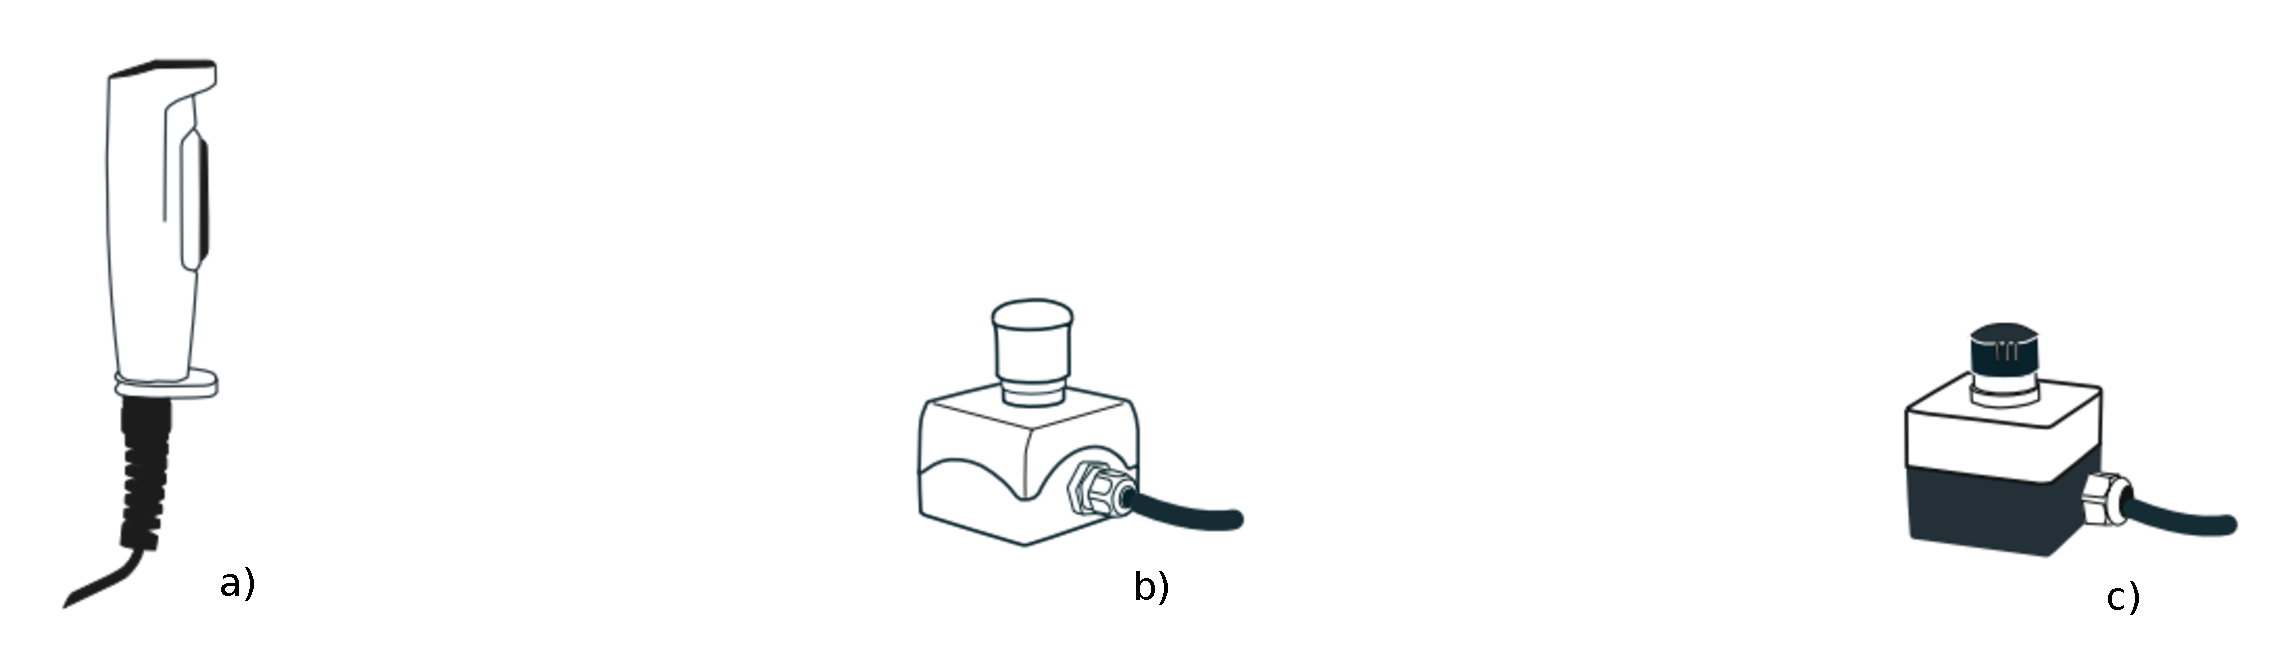
\includegraphics[width=\textwidth]{panda_safety_devices}
	\caption{Panda safety devices. (a) External enabling device; (b) External activation device; (c) Emergency stop device. Courtesy of Franka Emika GmbH and adapted from Panda user handbook of 2018.}
	\label{fig:panda_safety_devices}
\end{figure}

% subsection robotic_system_physical_description_safety_devices

\subsection*{Host PC}
\label{subsec:robotic_system_physical_description_hostpc}

The Host PC is the computer that the robot operator uses to access the Desk interface and run the custom controllers code. This computer should be connected directly to Control if using \gls{fci}, otherwise it can be connected directly to the Panda Arm. To use Desk, the computer only needs an ethernet port and a web browser. To use \gls{fci}, the computer also needs to be running a real time operating system kernel, and have the CPU in performance mode. The preparation of the Host PC to operate under \gls{fci} will be described on the section \ref{sec:robotic_system_integration_ros}.

% subsection robotic_system_physical_description_hostpc

% section robotic_system_physical_description

% ==========================
% = Operation =
% ==========================

\section{Operation}
\label{sec:robotic_system_operation}

\subsection{Installation}
\label{subsec:robotic_system_operation_installation}

% subsection robotic_system_operation_installation

\subsection{Security}
\label{subsec:robotic_system_operation_security}

% subsection robotic_system_operation_security

\subsection{Operation with Desk}
\label{subsec:robotic_system_operation_desk}

% subsection robotic_system_operation_desk

% section robotic_system_operation

% ==========================
% = Integration with ROS =
% ==========================

\section{Integration with \gls{ros}}
\label{sec:robotic_system_integration_ros}

% section robotic_system_integration_ros

% ==========================
% = Integration with Gazebo =
% ==========================

\section{Integration with Gazebo}
\label{sec:robotic_system_integration_gazebo}

% section robotic_system_integration_gazebo